\documentclass[a4paper]{report}%{book}

\usepackage{amsmath} % assumes amsmath package installed
\usepackage{amssymb}  % assumes amsmath package installed
\usepackage{graphicx}
\usepackage{lettrine}
\usepackage{natbib}
%\usepackage{biblatex}
\usepackage{wrapfig}
\usepackage{color}
\usepackage{caption}
\usepackage{titlesec}
%\usepackage{subfigure}
\usepackage[raggedright]{sidecap}
\usepackage[table]{xcolor}
\usepackage{changepage}
\usepackage{tikz-cd}
\usepackage{algorithm}
%\usepackage{algorithmic}
\usepackage[noend]{algpseudocode}
%\usepackage{subcaption}
\usepackage{xcolor}

\usepackage[titletoc]{appendix}

% Consente di definire in modo flessible note e titoli
\usepackage{fancyhdr}
\pagestyle{fancy} 

\usepackage{calc}

\usepackage{makecell}
\usepackage{subfig}
\newcommand{\NE}{\mathbfsymbol{\rm{NE}}}
\newcommand{\sbt}{\,\begin{picture}(-1,1)(-1,-3)\circle*{3}\end{picture}\ }
\def\Real{\mathbb{R}}
\def\tm{\leavevmode\hbox{$\rm {}^{TM}$}}
\def\Complex{\mathbb{C}}
\usepackage{mathtools}
\newcommand\numberthis{\addtocounter{equation}{1}\tag{\theequation}}
\usepackage{array}
\newcolumntype{P}[1]{>{\centering\arraybackslash}p{#1}}
\newcolumntype{M}[1]{>{\centering\arraybackslash}m{#1}}
\usepackage{lipsum}
\renewcommand\theadalign{cb}
\renewcommand\theadgape{\Gape[4pt]}
\renewcommand\cellgape{\Gape[4pt]}
\usepackage{color}

\usepackage[font=small]{caption}
%\newcommand*\subsectotoc[1]{\subsection*{#1}\addcontentsline{toc}{subsection}{#1}}

\graphicspath{{Figures/}}

\fancyheadoffset[LE,RO]{\marginparsep+\marginparwidth} 
\renewcommand{\chaptermark}[1]{\markboth{#1}{}} 
\renewcommand{\sectionmark}[1]{\markright{\thesection\ #1}} 
\fancyhf{}
\fancyhead[LE,RO]{\color{black}\bfseries\thepage} 
\fancyhead[LO]{\color{black}\bfseries\rightmark} 
\fancyhead[RE]{\color{black}\bfseries\leftmark} 


% Con questo comando si dice a LaTex dove sono memorizzate le figure
%\graphicspath{{./imgs/}}
\newcommand{\folder}{./file/}

\usepackage[Bjornstrup]{fncychap}

\definecolor{redSapienza}{RGB}{160, 36, 41}

\colorlet{partbgcolor}{gray!10}% shaded background color for parts
\colorlet{partnumcolor}{black}% color for numbers in parts
\colorlet{chapbgcolor}{gray!15}% shaded background color for chapters
\colorlet{chapnumcolor}{black}% color for numbers in chapters

\renewcommand\DOCH{%
  \settowidth{\py}{\CNoV\thechapter}
  \addtolength{\py}{-10pt}
  \fboxsep=0pt%
  \colorbox{chapbgcolor}{\rule{0pt}{40pt}\parbox[b]{\textwidth}{\hfill}}%
  \kern-\py\raise20pt%
  \hbox{\color{chapnumcolor}\CNoV\thechapter}\\%
}

\renewcommand\DOTI[1]{%
  \nointerlineskip\raggedright%
  \fboxsep=\myhi%
  \vskip-1ex%
  \colorbox{chapbgcolor}{\parbox[t]{\mylen}{\CTV\FmTi{#1}}}\par\nobreak%
  \vskip 40pt%
}

\renewcommand\DOTIS[1]{%
  \fboxsep=0pt
  \colorbox{chapbgcolor}{\rule{0pt}{40pt}\parbox[b]{\textwidth}{\hfill}}\\%
  \nointerlineskip\raggedright%
  \fboxsep=\myhi%
  \colorbox{chapbgcolor}{\parbox[t]{\mylen}{\CTV\FmTi{#1}}}\par\nobreak%
  \vskip 40pt%
 }
\makeatother

\ChTitleVar{\hfill  \it \bf \huge \color{black}}
\ChNumVar{\fontsize{76}{80}\usefont{OT1}{pzc}{m}{n}\selectfont \color{redSapienza}}

\usepackage{bookmark,hyperref}
\hypersetup{pdfborder=0 0 0}
\hypersetup{colorlinks=true,linkcolor=black}
\hypersetup{citecolor=red}

\pdfinfo{
   /Author (Milad Kiwan)
   /Title  (Title)
   /CreationDate (March 2020)
   /Subject (Computer science)
}

%% requirements
\usepackage{amsmath}

%%%%%%%%%%%%%%%%%%%%%%%%%%%%%%%%%%%%%%%%%%%%%%%%%%%%%%%%%%%%%
%%%%%%%%%%%%%%%%% Allgemeines %%%%%%%%%%%%%%%%%%%%%%%%%%%%%%%%

\newcommand{\sign}{\operatorname{sign}}

%\newcommand{\Real}{\mathbb{R}}

% Allgemeine Vektor-Matrix-Definitionen
\newcommand{\vect}[1]{\boldsymbol{#1}}
\newcommand{\mat}[1]{\boldsymbol{#1}}

\newcommand{\diff}[2]{\frac{\partial #1}{\partial #2}}
\newcommand{\diffs}[3]{\frac{\partial^2 #1}{
\ifx#2#3 
\partial #2^2
\else
\partial #2 \partial #3
\fi
}}
%\newcommand{\norm}[1]{{\left \| {#1} \right \|}}
\newcommand{\de}[1]{{\left | {#1} \right |}}

%\newcommand{\dddott}[1]{{#1}^{[3]}}
\newcommand{\dddott}[1]{{\stackrel{\boldsymbol{...}}{#1}}}
%\newcommand{\ddddott}[1]{{#1}^{[4]}}
\newcommand{\ddddott}[1]{{\stackrel{\boldsymbol{....}}{#1}}}

%%%%%%%%%%%%%%%%%%%%%%%%%%%%%%%%%%%%%%%%%%%%%%%%%%%%%%%%%%%%%%
%%%%%%%%%%%%%%%%% Vektoren und Matrizen %%%%%%%%%%%%%%%%%%%%%%

\newcommand{\zerov}{\vect{0}}

%%%%%%%%%%%%%%%%%%%%%%%%%%%%%%%%%%%
%%% Vektoren - Kleinbuchstablen %%%
%%%%%%%%%%%%%%%%%%%%%%%%%%%%%%%%%%%

\newcommand{\av}{\vect{a}}
\newcommand{\bv}{\vect{b}}
\newcommand{\cv}{\vect{c}}
\newcommand{\dcv}{\dot{\vect{c}}}
\newcommand{\ddcv}{\ddot{\vect{c}}}
\newcommand{\dv}{\vect{d}}
\newcommand{\ev}{\vect{e}}
\newcommand{\dev}{\dot{\vect{e}}}
\newcommand{\ddev}{\ddot{\vect{e}}}
\newcommand{\fv}{\vect{f}}
\newcommand{\gv}{\vect{g}}
\newcommand{\gbv}{\bar{\vect{g}}}
\newcommand{\dgv}{\dot{\vect{g}}}
\newcommand{\ddgv}{\ddot{\vect{g}}}
\newcommand{\hv}{\vect{h}}
\newcommand{\iv}{\vect{i}}
\newcommand{\kv}{\vect{k}}
\newcommand{\lv}{\vect{l}}
\newcommand{\mv}{\vect{m}}
\newcommand{\nv}{\vect{n}}
\newcommand{\dnv}{\dot{\vect{n}}}
\newcommand{\ddnv}{\ddot{\vect{n}}}
\newcommand{\ov}{\vect{o}}
\newcommand{\pv}{\vect{p}}
\newcommand{\dpv}{\dot{\vect{p}}}
\newcommand{\ddpv}{\ddot{\vect{p}}}
\newcommand{\qv}{{\vect{q}}}
\newcommand{\dqv}{\dot{\vect{q}}}
\newcommand{\ddqv}{\ddot{\vect{q}}}
\newcommand{\dddqv}{\dddott{\vect{q}}}
\newcommand{\ddddqv}{\ddddott{\vect{q}}}
\newcommand{\qbv}{\bar{\vect{q}}}
\newcommand{\dqbv}{\dot{\bar{\vect{q}}}}
\newcommand{\ddqbv}{\ddot{\bar{\vect{q}}}}
\newcommand{\dddqbv}{\dddott{\bar{\vect{q}}}}
\newcommand{\ddddqbv}{\ddddott{\bar{\vect{q}}}}
\newcommand{\qhv}{\hat{\vect{q}}}
\newcommand{\qtbv}{\tilde{\bar{\vect{q}}}}
\newcommand{\rv}{{\vect{r}}}
\newcommand{\drv}{\dot{\vect{r}}}

\newcommand{\dq}{\dot{q}}
\newcommand{\ddq}{\ddot{q}}

%\newcommand{\rv}{\bar\qv}

\newcommand{\sv}{\vect{s}}
\newcommand{\dsv}{\dot{\vect{s}}}
\newcommand{\tv}{\vect{t}}
\newcommand{\uv}{\vect{u}}
\newcommand{\vv}{\vect{v}}
\newcommand{\dvv}{\dot{\vect{v}}}
\newcommand{\wv}{\vect{w}}
\newcommand{\dwv}{\dot{\vect{w}}}
\newcommand{\xv}{\vect{x}}
\newcommand{\dxv}{\dot{\vect{x}}}
\newcommand{\ddxv}{\ddot{\vect{x}}}
\newcommand{\dddxv}{\dddott{\vect{x}}}
\newcommand{\ddddxv}{\ddddott{\vect{x}}}
\newcommand{\txv}{\vect{\tilde{x}}}
\newcommand{\dtxv}{\dot{\tilde{\vect{x}}}}
\newcommand{\ddtxv}{\ddot{\tilde{\vect{x}}}}
\newcommand{\dddtxv}{\dddott{\tilde{\vect{x}}}}
\newcommand{\ddddtxv}{\ddddott{\tilde{\vect{x}}}}
\newcommand{\yv}{\vect{y}}
\newcommand{\ybv}{\bar{\vect{y}}}
\newcommand{\dyv}{\dot{\vect{y}}}
\newcommand{\ytv}{\tilde {\vect{y}}}
\newcommand{\zv}{\vect{z}}
\newcommand{\dzv}{\dot{\vect{z}}}
\newcommand{\ddzv}{\ddot{\vect{z}}}


%%%%%%%%%%%%%%%%%%%%%%%%%%%%%%%%%%%%%%%%%%%%%%%%
%%% Vektoren - Kleinbuchstablen - griechisch %%%
%%%%%%%%%%%%%%%%%%%%%%%%%%%%%%%%%%%%%%%%%%%%%%%%

\newcommand{\alphav}{\vect{\alpha}}
\newcommand{\varepsilonv}{\vect{\varepsilon}}
\newcommand{\betav}{\vect{\beta}}
\newcommand{\gammav}{\vect{\gamma}}
\newcommand{\Gammav}{\vect{\Gamma}}
\newcommand{\deltav}{\vect{\delta}}
\newcommand{\ddeltav}{\dot{\vect{\delta}}}

\newcommand{\phiv}{\vect{\phi}}
\newcommand{\varphiv}{\vect{\varphi}}
\newcommand{\dphiv}{\dot{\vect{\phi}}}
\newcommand{\ddphiv}{\ddot{\vect{\phi}}}

\newcommand{\psiv}{\vect{\psi}}

\newcommand{\sigmav}{\vect{\sigma}}
\newcommand{\dsigmav}{\dot{\vect{\sigma}}}

\newcommand{\tauv}{\vect{\tau}}
\newcommand{\dtauv}{\dot{\vect{\tau}}}
\newcommand{\ddtauv}{\ddot{\vect{\tau}}}
\newcommand{\thetav}{\vect{\theta}}
\newcommand{\dthetav}{\dot{\vect{\theta}}}
\newcommand{\ddthetav}{\ddot{\vect{\theta}}}
\newcommand{\thetavt}{\tilde {\vect{\theta}}}
\newcommand{\muv}{\vect{\mu}}
\newcommand{\nuv}{\vect{\nu}}
\newcommand{\omegav}{\vect{\omega}}
\newcommand{\xiv}{\vect{\xi}}
\newcommand{\dxiv}{\dot{\vect{\xi}}}
\newcommand{\piv}{\vect{\pi}}
\newcommand{\lambdav}{\vect{\lambda}}

%%%%%%%%%%%%%%%%%%%%%%%%%%%%%%%%%%%
%%% Vektoren - Grossbuchstablen %%%
%%%%%%%%%%%%%%%%%%%%%%%%%%%%%%%%%%%

\newcommand{\Av}{\vect{A}}
\newcommand{\Fv}{\vect{F}}
\newcommand{\Lv}{\vect{L}}
\newcommand{\Mv}{\vect{M}}
\newcommand{\Tv}{\vect{T}}
\newcommand{\Vv}{\vect{V}}
\newcommand{\Wv}{\vect{W}}

%%% Einheits-Matrix
\newcommand{\IIm}{\mat{I}}
%%% Null-Matrix
\newcommand{\zerom}{\mat{O}}

%%%%%%%%%%%%%%%%%%%%%%%%%%%%%%%%%%%
%%% Matrizen - Grossbuchstablen %%%
%%%%%%%%%%%%%%%%%%%%%%%%%%%%%%%%%%%

\newcommand{\Am}{\mat{A}}
\newcommand{\Bm}{\mat{B}}
\newcommand{\Cm}{\mat{C}}
\newcommand{\dCm}{\dot{\Cm}}
\newcommand{\ddCm}{\ddot{\Cm}}
\newcommand{\dddCm}{\dddott{\Cm}}
\newcommand{\Dm}{\mat{D}}
\newcommand{\Em}{\mat{E}}
\newcommand{\Fm}{\mat{F}}
\newcommand{\Gm}{\mat{G}}
\newcommand{\Hm}{\mat{H}}
\newcommand{\Jm}{\mat{J}}
\newcommand{\Lm}{\mat{L}}
\newcommand{\Jbm}{\bar{\mat{J}}}
\newcommand{\dJm}{\dot{\mat{J}}}
\newcommand{\ddJm}{\ddot{\Jm}}
\newcommand{\dddJm}{\dddott{\Jm}}
\newcommand{\Km}{\mat{K}}
\newcommand{\Mm}{\mat{M}}
\newcommand{\dMm}{\dot{\Mm}}
\newcommand{\ddMm}{\ddot{\Mm}}
\newcommand{\dddMm}{\dddott{\Mm}}
\newcommand{\Nm}{\mat{N}}
\newcommand{\Pm}{\mat{P}}
\newcommand{\Qm}{\mat{Q}}
\newcommand{\Rm}{\mat{R}}
\newcommand{\Sm}{\mat{S}}
\newcommand{\Tm}{\mat{T}}
\newcommand{\Um}{\mat{U}}
\newcommand{\Vm}{\mat{V}}
\newcommand{\Wm}{\mat{W}}
\newcommand{\Ym}{\mat{Y}}
\newcommand{\Zm}{\mat{Z}}

%%%%%%%%%%%%%%%%%%%%%%%%%%%%%%%%%%%%%%%%%%%%%%%%
%%% Matrizen - Grossbuchstablen - griechisch %%%
%%%%%%%%%%%%%%%%%%%%%%%%%%%%%%%%%%%%%%%%%%%%%%%%

\newcommand{\calAm}{\mat{\cal A}}
\newcommand{\calCm}{\mat{\cal C}}
\newcommand{\calMm}{\mat{\cal M}}
\newcommand{\calKm}{\mat{\cal K}}
\newcommand{\calEm}{\mat{\cal E}}
\newcommand{\dcalMm}{\dot{\calMm}}

\newcommand{\Deltam}{\mat{\Delta}}
\newcommand{\Gammam}{\mat{\Gamma}}
\newcommand{\Lambdam}{\mat{\Lambda}}
\newcommand{\mum}{\mat{\mu}}
\newcommand{\Sigmam}{\mat{\Sigma}}
\newcommand{\Thetam}{\vect{\Theta}}
\newcommand{\dThetam}{\dot{\Thetam}}
\newcommand{\ddThetam}{\ddot{\Thetam}}

%%%%%%%%%%%%%%%%%%%%%%%%%%%%%%%%%%%%%%%%%%%%%%%%
%%% Matrizen - mit indizes                   %%%
%%%%%%%%%%%%%%%%%%%%%%%%%%%%%%%%%%%%%%%%%%%%%%%%

\newcommand{\Jqm}{\Jm_{f_q,q}}
\newcommand{\Jtm}{\Jm_{f_q,\theta}}
\newcommand{\Jqbm}{\Jm_{\bar q}}
\newcommand{\Jgm}{\Jm_{g}}
\newcommand{\Jhm}{\Jm_{h}}
\newcommand{\xbv}{\thetav,\qbv(\thetav)} 



%%%%%%%%%%%%%%%%%%%%
% figures
%%%%%%%%%%%%%%%%%%%%
%IMAGE DEFINITION
\def\autoencoder{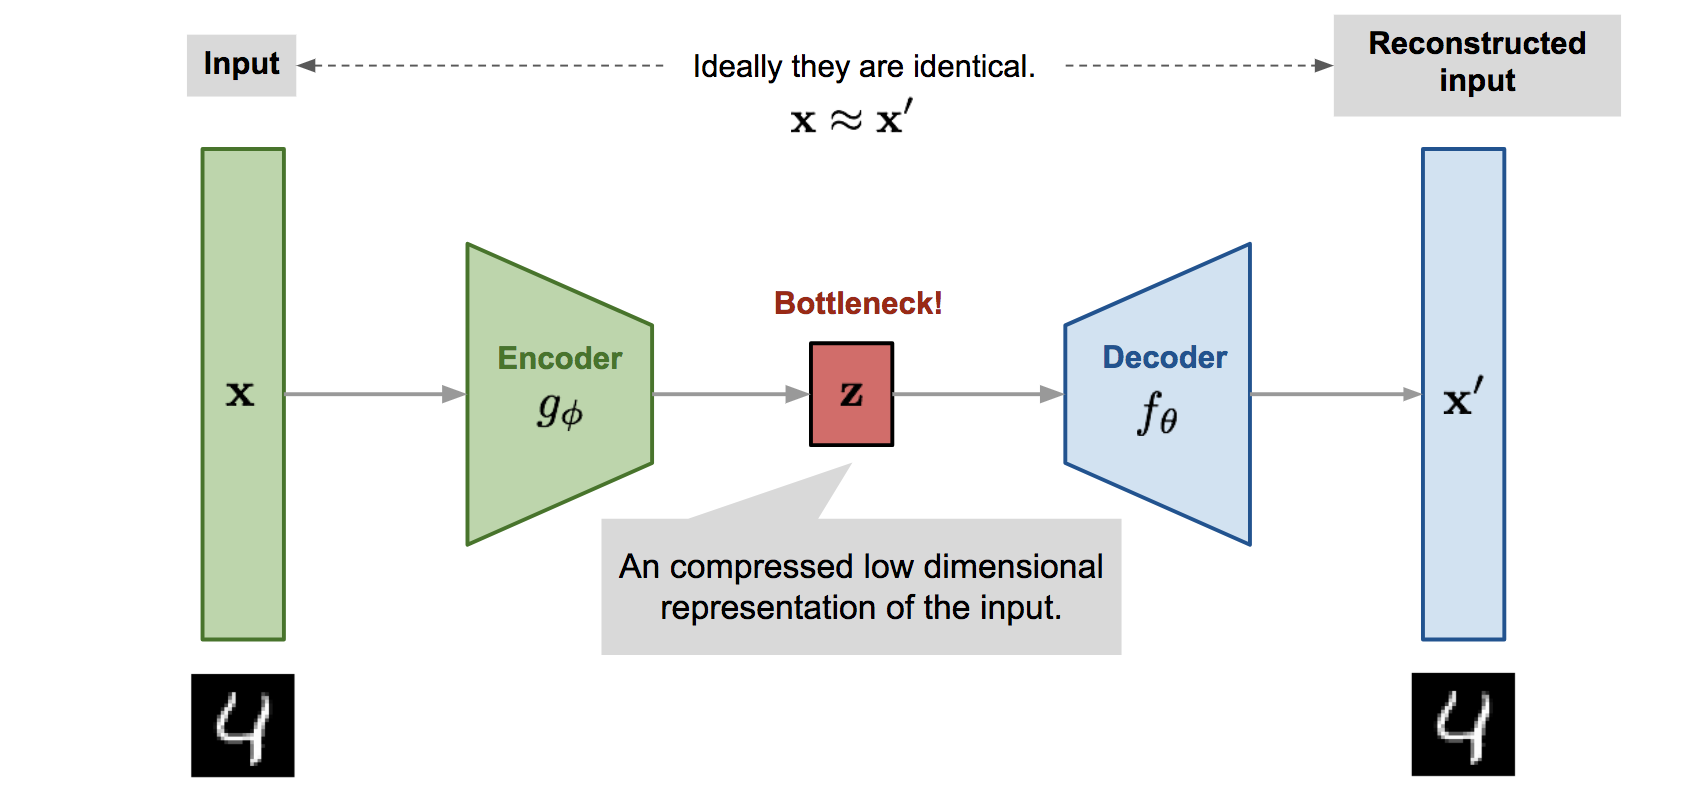
\includegraphics[scale=0.4]{autoencoder-architecture.png}}
\def\paratrick{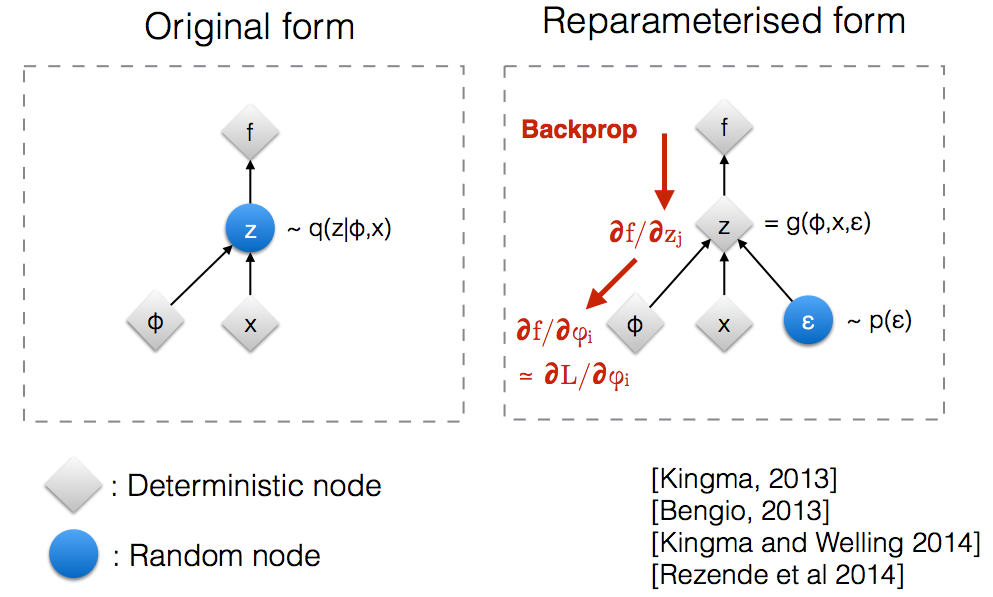
\includegraphics[scale=0.4]{para_trick.png}}




%%%%%%%%%%%%%%%%%%%%

\begin{document}

%Con queto comando si pu� cambaire il modo in cui verranno nominate le
	%figure. Di default � "Figura", qui viene cambiato in "Fig."
	%\renewcommand{\figurename}{Fig.}

	% === Frontespizio =======================================
	% formato della pagina: l'argomento empty sta ad indicare che sia le linee
	% di testa che quelle di coda sono vuoti e non hanno numeri di pagina
	\pagenumbering{roman}
	% Frontespizio: mediante il comando input si legge il frontespizio
	%%%%%%%%%%%%%%%%%%%%%%%%%%%%%%%%%%%%%%%%%%%%%%%%%%%%%%%%%%%
% Frontespizio

% vspace serve ad aggiungere extra spazio verticale
% em sta ad indicare la grandezza della lettera M maiuscola

% Large indica una dimensione del font di 14.4 pt
% large indica una dimensione del font di 12 pt
% normalsize indica una dimensione del font di 10 pt

% vfill inserisce sufficiente spazio binaco verticalmente per fare in modo che il
% sopra e il sotto del testo siano allieneati col margine superiore e inferiore

\hypersetup{pdftitle={Usage example of the Sapthesis class for a Laurea Magistrale thesis in English},pdfauthor={Milad Kiwan}}

% Remove in a normal thesis
%\definecolor{gray}{gray}{0.4}
\definecolor{black}{rgb}{0.0, 0.0, 0.0}
\newcommand{\bs}{\textbackslash}

% Commands for the titlepage
\title{State Of Art Of Generative Models in robotics\\ Applications\\ Master thesis in engineering in computer science}
\author{Milad Kiwan}
\IDnumber{1164659}
\course{Ingegneria Informatica}
\courseorganizer{Facolt\`{a} Ingegneria dell'informazione, informatica e statistica}
\AcademicYear{2019/2020}
\copyyear{2020}
\advisor{Prof. Daniele Nardi}
\advisor{Dr. Francesco Riccio}
%\coadvisor{Dr. Nome Cognome}
\authoremail{miladkiwan@hotmail.com}

\examdate{20 April 2020}
\examiner{Prof. Lenzerini Maurizio}
\examiner{Prof. Nardi Daniele}
\examiner{Prof. Giorgio Grisetti}
\examiner{Prof. Comminiello Danilo}
\examiner{Prof. Massimo	Mecella}
\examiner{Dr. Scardapane Simone}
\examiner{Dr. Anagnostopoulos Aristidis}
\versiondate{\today}


\maketitle

%\clearpage{\pagestyle{empty}\cleardoublepage}

%%%%%%%%%%%%%%%%%%%%%%%%%%%%%%%%%%%%%%%%%%%%%%%%%%%%%%%%%%%
%% Scheda Interna
%
%\begin{titlepage}
% \begin{center}
%     \includegraphics[width=6cm]{logob}\\
%     \vspace{1em}
%     {\Large \textsc{Universit� degli studi di Roma "La Sapienza"}}\\
%     \vspace{1em}
%     {\Large \textsc{Facolt� di Ingegneria}}\\
%     \vspace{2em}
%     {\normalsize Tesi di Laurea in}\\
%     \vspace{1em}
%     {\Large \textsc{Ingegneria Elettronica}}\\
%     \vspace{5em}
%     {\LARGE \textbf{Interazione uomo-robot mediante comandi gesturali e vocali}}\\
% \end{center}
%
%\vskip 2.5cm
%  \begin{center}
%    \begin{tabular}{l c c c c c c l}
%      \large \textbf{Relatore} & & & & & & & \large \textbf{Candidato} \\[0.2cm]
%      \large{Prof. Alessandro De Luca} & & & & & & & \large{Emanuele Magrini}\\[0.4cm]
%       \large \textbf{Correlatore} & & & & & & & \\[0.2cm]
%      \large{Dott. Fabrizio Flacco}& & & & & & & \\
%    \end{tabular}
%  \end{center}
%
%\vskip 2cm
%\begin{center}
%{\normalsize Anno Accademico 2011/2012}
%\end{center}
%\end{titlepage}
\clearpage{\pagestyle{empty}\cleardoublepage}

%%%%%%%%%%%%%%%%%%%%%%%%%%%%%%%%%%%%%%%%%%%%%%%%%%%%%%%%%%%
% Dedica

\vspace{5em}
% \begin{flushright}
% {\Large \textit{to my family and friends}}
% \end{flushright}

\pagestyle{empty}
	
\begin{center}
	%\thispagestyle{empty}
	%\vspace*{\fill}
%{\em To my both colleague and wife, Maram, \\ \qquad \qquad \quad  and to my daughter, Yafa.}
	%{\em To my family.}
	{\em Dedication.}
	%\vspace*{\fill}
\end{center}

%\begin{flushright}
%\vspace*{\fill}
%	To my beloved Mara
%	\vspace*{\fill}
%\end{flushright}

\clearpage{\pagestyle{empty}\cleardoublepage}
	%%%%%%%%%%%%%%%%%%%%%%%%%%%%%%%%%%%%%%%%%%%%%%%%%%%%%%%%%%%
% Abstract
\pagestyle{fancy}

\providecommand{\keywords}[1]{\textbf{Keywords:} #1}

\chapter*{Abstract}
\addcontentsline{toc}{chapter}{Abstract}

\vspace{-30 pt}



\keywords{\textit{Generative models, Generative Adversarial Networks, Reinforcement Learning, Variational Autoencoders, Robotics}}\\

This thesis makes an overview on the most used architectures that have been designed to achieve generative models, and show some of the recent frameworks and algorithms in robotics applications that make use of these generative models. It presents as well how these models assisted the existing frameworks like reinforcement learning that had the lead in succession in robotics applications in the last years. The combination between generative models and reinforcement learning in problems like imitation learning and learn from demonstration has led to achieve better performing frameworks. 

\clearpage{\pagestyle{empty}\cleardoublepage}






	%%%%%%%%%%%%%%%%%%%%%%%%%%%%%%%%%%%%%%%%%%%%%%%%%%%%%%%%%%%
% Acknowledgements

\pagestyle{fancy}
\chapter*{Acknowledgements}
\addcontentsline{toc}{chapter}{Acknowledgements}

Firstly, I would like to express my sincere gratitude to my teacher and advisor Prof. Daniele Nardi and his assistent Francesco Riccio for the sustained support of my masters study and related research, motivation, and immense knowledge. 

\vspace{5pt}
Also, I would like to thank all my friends for their motivation and nice refresh breaks during the day. 

\vspace{5pt}
A big thanks to my parents for their endless encouragement, support, and patience for being far from them.

\clearpage{\pagestyle{empty}\cleardoublepage}


\tableofcontents
\clearpage{\pagestyle{empty}\cleardoublepage}

%\listoffigures
 
%\listoftables

\pagenumbering{arabic}

%%%%%%%%%%%%%%%%%%%%%%%%%%%%%%%%%%%%%%%%%%%%%%%%%%%%%%%%%%%
% Introduction
%\clearpage{\pagestyle{empty}}

\pagestyle{fancy}  
\chapter*{Introduction}
\addcontentsline{toc}{chapter}{Introduction}
\vspace{5 pt}
There is an immense effort in machine learning and statistics to develop accurate and scalable probabilistic models of data. Such models are called upon whenever we are faced with tasks requiring probabilistic reasoning, such as prediction, missing data imputation and uncertainty estimation; or in simulation-based analyses, common in many scientific fields such as genetics, robotics and control that require generating a large number of independent samples from the model. The benefit of employing a generative model lies in its wide applicability to the problem of inference. For example, many robotic tasks include the problem of evaluating the likelihood of an observation of the environment given some piece of relevant information, such as the location of the camera, a particular object model hypothesis, or even raw images. However, generative models in robotics are used to solve various issues faced during the implementation of applications in robotics field to design intelligent machines that can help and assist humans in their day-to-day lives. Such as learn from demonstrations or sometimes called imitation learning, which is a paradigm for enabling robots to autonomously perform new tasks, help reinforcement learning to learn from high-dimensional state space, lean wild set of tasks, and improve polices either with or without demonstrations. The lack of data as well is one of the main efficiency and stability is one of the main challenges in end-to-end methods like those of\textit{ \textacutedbl reinforcement learning\textgravedbl.} It is hard to talk about robotics without mention reinforcement learning, which as a field, has had the major success in past few years. RL offers to robotics a set of tools and algorithms that can assist to design complicated robotic behavior to achieve sophisticated tasks. More recently, another field in machine learning that had the lead in success well as is\textit{ \textacutedbl Generative Adversarial Networks\textgravedbl} this great idea of gaming networks, invented by Ian Goodfellow, has been exploit in RL to achieve more complicated frameworks that, as we will see later in this work.
\\During this work we will talk about the main techniques and algorithms used to perform generative models that have assisted the robotics applications to achieve the respective tasks, and go through some of the frameworks and papers that we deemed most interesting, and showed the importance role the generative modeling plays in the most recent robotics applications. Afterward we will discuss these frameworks explaining their functioning and how the generative models were employed to become useful in the various settings. Then we will show the results obtained from this employment, and argue the effects and the limits on these applications. At the end we will talk about the conclusions extracted during the extension of this survey, and offer some thoughts about how might the generative models in robotics extend and where would be the direction of the future works.


\clearpage{\pagestyle{empty}\cleardoublepage}

%\part{Part I}
%%%%%%%%%%%%%%%%%%%%%%%%%%%%%%%%%%%%%%%%%%%%%%%%%%%%%%%%%%%
% Chapter1


\pagestyle{fancy} 
\chapter{Variational Auto-Encoder (VAEs)}
\label{cha:1}
\vspace{1cm}


\section{Introduction}
\label{sec:}
One of the reasons for which the generative models have been employed in different type of applications is the powerful and utility of VAE, where they are used to either solve issues in AI like image reconstruction and generation, achieve better results, reduce the computational complexity due to the high dimensionality of the data, find latent space, reduce dimensionality, extract and represent features or learn density distribution of the dataset. In this session it’s given an overview on how a VAE network is structured and what are the main techniques applied to make it useful to each of the issues just mentioned above.
\vspace{0.3cm}

\section{VAE Structure}
Before starting to talk about the usage VAEs, it is mandatory to go through the structure of the auto-encoder which is essentially a neural network with a bottleneck in the middle Fig~\ref{fig:autoencoder} designed to reconstruct the original input in an unsupervised way, in other words, it learns an identity function by first reducing the dimension of the data to the bottleneck so as to extract more efficient and compressed representation. Surprisingly The idea was originated in the 1980s, and later promoted by the seminal paper by~\cite{hinton2006reducing}.

\vspace{0.3cm}
The Auto-Encoder consists of tow connected networks that could be any kind of neural networks (convolutional, or multi-layer perceptron etc) depends on the data it has to deal with, which are:
\begin{itemize}
	\item Encoder network: gets the high-dimension input and transform it to into a low-dimension code in the bottleneck, or we can call it representation, latent or features as well again depends on what the usage are we making of the auto-encoder.
	\item Decoder network: gets the output of the encoder and does essentially the inverse process, or we can say reconstruct the data, likely with larger and larger layers to the last one that outputs the reconstructed original data.
\end{itemize}

\begin{figure}
	\centerline
	\autoencoder
	\caption{Autoencoder}
	\label{fig:autoencoder}
\end{figure} 

We can see already how the auto-encoder networks can give us an efficient way to  impressively represent the data and in lower dimension. So the accomplishment of solutions for the problematics we talked about at beginning of this session, is all about about how we build the bottleneck layer or what will call from now on vector $z$. The VAE~\cite{kingma2013auto} basically is an auto-encoder but the structure of vector $z$ is quite different. For instance what if we need to map the input into a probability distribution $q_{\theta}$ instead of a fixed vector $z$, where $q_{\theta}$ is parameterized by $\theta$, from which we sample or generate $z$, this is what make the VAE to be recognized as a generative model. Where the training is regularized to avoid eventual overfitting  that might occur with auto-encoder architecture and ensure that the distribution $q_{\theta}$ has good parameters to enable the generative process. The way that makes the encoder to be able to produce $q_\theta$ is by composing the bottleneck or the output of a mean $\mu$ and a covariance matrix $\Sigma$ the problem here is that nothing would prevent the this distribution to be extremely narrow, or effectively a single value. To escape the issue, the Kullback–Leibler (KL) divergence-which measures the distance between tow distributions- is introduced  between the distribution produced by the encoder $q_{\theta}(z \mid x_i)$ and a unit Gaussian distribution $p(z)$(mean $0$, covariance matrix is the identity matrix) and tell us how much information is lost when using q to represent p, this KL divergence is then introduced as a penalty to the loss function li, which consists of another term as well that is the expected negative likelihood of the $i$-th datapoint $x_i$ as follow:


\begin{equation}
l_i(\theta,\phi)=-E_{z\sim q_\theta (z\mid x_i)}[\log_{p_\phi}(x_i \mid z)]+KL(q_\theta (z\mid x_i)||p(z))
\label{eq:VAE_loss}
\end{equation}
Where $z$ is sampled from $q_\theta$ and $\phi$ the decoder parameters, the purpose of the first term in poor words mean “how much the decoder output is similar to original datapoint $x_i$“. It intuitively leads the decoder to learn to reconstruct the data. The last important part left to talk about is the training one, we can use the gradient descent to optimize the loss with respect to the parameters of the encoder and decoder $\theta$ and $\phi$ respectively. For stochastic gradient descent with step size $\rho$, the encoder parameters are updated using $\theta=\theta-\frac{\partial l}{\partial \theta} $  and the decoder is updated similarly.



\subsection{Reparameterization Trick:}
As we can notice at this point that there would be a problem doing the backpropagation step of the gradient descent optimizer, because it does not go through the random node z, therefore we have to implement some trick to circumvent this issue. The reparameterization trick~\cite{kingma2013auto} is essentially done by introducing an auxiliary variable (noise) $\varepsilon$ that allows us to reparameterize $z$ in a way that allows backpropagate to flow through the deterministic nodes as shown in Fig.~\ref{fig:paratrick}, we are basically expressing the random variable $z$ as a deterministic 

\begin{figure}
	\centerline
	\paratrick
	\caption{reparameterization trick}
	\label{fig:paratrick}
\end{figure} 


%\vspace{1cm}
\section{Employment of VAEs in generative models for robotics}
\label{sec:VAE_generative}
Lets go now through some papers to see where and how the VAEs have been employed and show their effectiveness in various applications of generative models in robotics. The first one~\cite{eslami2016attend} where a framework called by the authors "Attend, infer, repeat" (AIR) the VAE structure here is quite different that the encoder was implemented as a Recurrent Neural Network (RNN), since its purpose is to learn to detect and generate objects, specifically “where is the objects, what are they and how many are they”. The additional recurrence to the structure is basically to detect how many objects are present in the input data. Experiments were designed initially on 2D data particularly on multiple MNIST digits, and reliably the model were able to detect and generate the constituent digits from scratch, it shows advantages over state-of-art generative models computationally and also in terms of generalization to unseen datasets. Other Experiments on 3D datasets, considering scenes consisting of only one of three objects: a red cube, a blue sphere, and a textured cylinder. The network accurately and reliably infers the identity and pose of the object, on the other hand, an identical network trained to predict the ground-truth identity and pose values of the training data has much more difficulty in accurately determining the cube’s orientation.\\


Moreover, in robotics, grasping and manipulation of various objects is a critical and challenging problem,~\cite{veres2017modeling} has proposed another concept referred to as the grasp motor image (GMI) that combines
object perception and a learned prior over grasp configurations, to synthesize new grasps to apply to a different object. At the core of GMI is the autoencoder structure, taking advantage of Deep  Learning (DL), particularly building both encoder and decoder as Convolutional Neural Networks (CNN). The approach followed is intuitive: based on
perceptual information about an object, and an idea of how an object was previously grasped, collecting a object/grasp pair dataset of successful, cylindrical precision
robotic grasps using the V-REP simulator~\cite{rohmer2013v}, and object files provided by~\cite{kleinhans2015g3db} on a simulated “picking” task. The VAE was trained on this dataset to generate grasps for novel objects. GMI integrates
perceptual information and grasp configurations using deep generative models. Applying it to a simulated grasping task, has demonstrated the capacity of these models to transfer learned knowledge to novel objects under varying
amounts of available training data.\\





\clearpage{\pagestyle{empty}\cleardoublepage}
%\part{Part II}
%%%%%%%%%%%%%%%%%%%%%%%%%%%%%%%%%%%%%%%%%%%%%%%%%%%%%%%%%%%
% Chapter2


\pagestyle{fancy} 
\chapter{Generative Modeling in Robotics}
\label{cha:2}
\vspace{1cm}



\clearpage{\pagestyle{empty}\cleardoublepage}
%%%%%%%%%%%%%%%%%%%%%%%%%%%%%%%%%%%%%%%%%%%%%%%%%%%%%%%%%%%
% Chapter3


\pagestyle{fancy} 
\chapter{Discussion}
\label{cha:3}
\vspace{1cm}

\section{Employment of VAEs in generative models for robotics}
\label{sec:VAE_generative}
Lets go now through some papers to see where and how the VAEs have been employed and show their effectiveness in various applications of generative models in robotics. The first one~\cite{eslami2016attend} where a framework called by the authors \textsl{Attend, infer, repeat (AIR)} the VAE structure here is quite different that the encoder was implemented as a Recurrent Neural Network (RNN), since its purpose is to learn to detect and generate objects, specifically “where is the objects, what are they and how many are they”. The additional recurrence to the structure is basically to detect how many objects are present in the input data. Experiments were designed initially on 2D data particularly on multiple MNIST digits, and reliably the model were able to detect and generate the constituent digits from scratch, it shows advantages over state-of-art generative models computationally and also in terms of generalization to unseen datasets. Other Experiments on 3D datasets, considering scenes consisting of only one of three objects: a red cube, a blue sphere, and a textured cylinder. The network accurately and reliably infers the identity and pose of the object, on the other hand, an identical network trained to predict the ground-truth identity and pose values of the training data has much more difficulty in accurately determining the cube’s orientation.\\

Moreover, in robotics, grasping and manipulation of various objects is a critical and challenging problem,~\cite{veres2017modeling} has proposed another concept referred to as the grasp motor image (GMI) that combines object perception and a learned prior over grasp configurations, to synthesize new grasps to apply to a different object. At the core of GMI is the autoencoder structure, taking advantage of Deep  Learning (DL), particularly building both encoder and decoder as Convolutional Neural Networks (CNN). The approach followed is intuitive: based on
perceptual information about an object, and an idea of how an object was previously grasped, collecting a object/grasp pair dataset of successful, cylindrical precision robotic grasps using the V-REP  simulator~\cite{rohmer2013v}, and object files provided by~\cite{kleinhans2015g3db} on a simulated “picking” task. The VAE was trained on this dataset to generate grasps for novel objects. GMI integrates
perceptual information and grasp configurations using deep generative models. Applying it to a simulated grasping task, has demonstrated the capacity of these models to transfer learned knowledge to novel objects under varying amounts of available training data.\\


\section{Exploitation of VAE and GMM in RL}
As mentioned in the previous section, most of the time applying RL algorithm directly on high-dimensional data does not lead to a good performance, so in the kind of situation it is advantageous to make use of the techniques that permit to reduce the dimensionality by representing the data in more suitable way.\\

One of the frameworks I went through has exploit both VAE and GMM to neatly which makes it feasible to fit the dynamics
even when the number of samples is much lower than the
dimensionality of the system. this what~\cite{finn2016deep} does, where initially RL algorithm run on robot with initial random policy to collect N (5 for that experiment) samples, then use them to fit GMM to learn the environment dynamics  or the policy controller without vision but using only the robot’s configuration as the state. In a second phase a VAE is trained to encode image dataset with unsupervised learning to produce a low-dimensional bottleneck vector that is a natural choice for learned feature representation or feature points for each image that concisely describes the configuration of objects in the scene, the interesting part of this VAE is that it is forced to encode spatial features rather than values. This is obtained  basically by applying spatial soft-max activation function that consists of tow operations on the last convolutional layer of the encoder as follow:
\begin{equation}
s_{cij} = \frac {e^{\frac{a_{cij}}{\alpha}}}
{\sum_{\acute{i}\acute{j}} e^{ \frac {a_{c \acute{i} \acute{j}}}{\alpha}}}
\end{equation}
where the temperature $\alpha$ is a learned parameter. Then, the expected
2D position of each softmax probability distribution $s_c$ is
computed according to:
\begin{equation}
f_c = (\sum_i i ∗ s_{cij} , \sum_j j ∗ s_{cij} )
\end{equation}
which forms the autoencoder's bottleneck and essentially it is the learned spatial feature point representation, that will therefore be capable of directly localizing objects in the image. The third and final phase of this framework is same as the first one, but the difference here is that the controller is trained on the feature points of the encoder using same trajectory-centric reinforcement
learning algorithm.\\
The experiments of this method showed that it could be used to learn a wild range of manipulation skills that require close coordination between perception and
action, and uses a spatial feature representation of the environment, which is learned as a bottleneck layer in
an autoencoder. This allows us to learn a compact state from high-dimensional real-world images. Furthermore, since this
representation corresponds to image-space coordinates of objects in the scene, it is particularly well suited for continuous control. The trajectory-centric RL algorithm we employ can learn a variety of manipulation skills with these spatial
representations using only tens of trials on the real robot.\\

In another work~\cite{nair2018visual} a RL framework was designed to jointly learns representations and policies from raw sensor inputs that achieve arbitrary goals under this representation by practicing to reach self-specified random goals during training. Here shows up the problem of choosing a suitable goal representations, to deal with this, a goal space \c{G} as to be same as the state space \c{S}. As well the problem of high-dimensional observations such as images arises, to handle it the authors once again the rely on VAE to learn a latent embedding for both \c{G} and \c{S}, by executing a random policy to collect state observation and optimize Eq.~\ref{eq:VAE_loss}, an additional online training has been introduced where the VAE is fine-tuned during the policy training each 3000 environment steps on all of the images observed by the policy, because as the policy improve it might visit new state observations where the VAE is not trained on, this additional training helped the performance of the overall algorithm. The final step is to run the RL algorithm which is a value-based one in this work twin delayed deep deterministic
policy gradients (TD3)~\cite{fujimoto2018addressing} is used, the thing that should be pointed out here that the negative Mahalanobis distance in the latent space were used as a reward function, but it turned out that minimizing this squared distance was equivalent to maximize the probability of the latent goal. This framework for learning general-purpose goal-conditioned policies that can achieve goals specified with target observations.\\




\clearpage{\pagestyle{empty}\cleardoublepage}
%%%%%%%%%%%%%%%%%%%%%%%%%%%%%%%%%%%%%%%%%%%%%%%%%%%%%%%%%%%
% Chapter3


\pagestyle{fancy} 
\chapter{Generative Adversarial Networks (GANs)}
\label{cha:4}
\vspace{1cm}
\section{What is a GAN}

Generative adversarial networks (GAN) is algorithmic architecture that uses two neural networks, pitting one against the other (thus the “adversarial”) in order to generate new, synthetic instances of data that can pass for real data. They are used widely in image generation, video generation and voice generation. it was introduced firstly by~\cite{goodfellow2014generative} to create a new framework for estimating generative models via an adversarial process that corresponds to tow-player game,
the tow networks could have arbitrary architecture and they are trained simultaneously, one neural network, called the discriminator, is designed as classifier network to evaluate the authenticity  distinguishing between fake and real data instances, while the other one, called generator, is trained to generate data as close to the authentic ones. Meanwhile, the generator is creating new, synthetic instances that it passes to the discriminator. It does so in the hopes that they, too, will be deemed authentic, even though they are fake. The goal of the generator is to generate passable instances to lie without being caught. The goal of the discriminator is to identify those coming from the generator as fake. GANs are a clever way to train a generative model in the same manner of a supervised learning problem.

\section{GAN Algothim overview}
\label{sec:GAN_algorithm}
To describe the GAN algorithm Fig.~\ref{fig:GAN} it is possible to start from either the generator, or the discriminator, because as mentioned in the previous section it corresponds to a tow-player game, like in chess, conventionally the while starts, but even if black starts that does not change the essence of the game. However, let's start with the more interesting one with is the generative model.\\

\begin{figure}
	\centerline
	\GAN
	\caption{GAN Architecture}
	\label{fig:GAN}
\end{figure} 
The generator model takes a fixed-length random noise vector as input or and generates a sample in the domain. The vector is drawn randomly from a Gaussian distribution, and the vector is used to seed the generative process. This vector space is referred to as a latent space, or a vector space comprised of latent variables. Latent variables, or hidden variables, are those variables that are important for a domain but are not directly observable. It is often referred to latent variables, or a latent space, as a projection or compression of a data distribution. That is, a latent space provides a compression or high-level concepts of the observed raw data such as the input data distribution. In the case of GANs, the generator model applies meaning to points in a chosen latent space, such that new points drawn from the latent space can be provided to the generator model as input and used to generate new and different output examples, 
after training, the generator model is kept and used to generate new samples. Sometimes, the generator can be repurposed as it has learned to effectively extract features from examples in the problem domain. Some or all of the feature extraction layers can be used in transfer learning applications using the same or similar input data. \\

The Discriminator Model takes an example from the domain as input (real or generated) and predicts a binary class label of real or fake (generated).The real example comes from the training dataset. The generated examples are output by the generator model. The discriminator is a normal (and well understood) classification model. After the training process, the discriminator model is discarded as we are interested in the generator.\\
The generator and the discriminator have different training processes, and it proceeds in alternating periods:
\begin{enumerate}
	\item The discriminator trains for one or more epochs.
	\item The generator trains for one or more epochs.
	\item Repeat steps 1 and 2 to continue to train the generator and discriminator networks.
\end{enumerate}

Indeed, as the generator improves with training, the discriminator get worse, because it becomes more difficult to recognize the authentic instances rather than the generated one, which means in accuracy terms that if the generator succeeds perfectly then the discriminator has a 50\% accuracy, same as flipping a coin to predict the label of the current instance.
This progression poses a problem for convergence of the GAN as a whole: the discriminator feedback gets less meaningful over time. If the GAN continues training past the point when the discriminator is giving completely random feedback, then the generator starts to train on junk feedback, and its own quality may collapse, which produces limited varieties of samples. Contrarily. If the discriminator gets too successful that the generator gradient vanishes and learns nothing.
Anyways, training GANs is noted as hard to obtain but still there several techniques to make the training more stable, which are out of the boundaries of this work. GANs try to replicate a probability distribution. They should therefore use loss functions that reflect the distance between the distribution of the data generated by the GAN and the distribution of the real data. Of course, there are tow loss functions for each of the tow networks as introduced in~\cite{goodfellow2014generative}, the generator tries to minimize the following function while the discriminator tries to maximize it:
\begin{equation}
E_x[\log{D(x)}] + E_z[\log{(1-D(G(z)))}]
\label{eq:GAN_loss}
\end{equation}

where $D(x)$ is the discriminator's estimate of the probability that real data instance x is real.
$E_x$ is the expected value over all real data instances. $G(z)$ is the generator's output when given noise z. $D(G(z))$ is the discriminator's estimate of the probability that a fake instance is real.
$E_z$ is the expected value over all random inputs to the generator (in effect, the expected value over all generated fake instances $G(z)$). The formula derives from the cross-entropy between the real and generated distributions. Since the generator can not directly affect $\log{D(x)}$ so, for the generator, minimizing the loss is equivalent to minimizing $log(1 - D(G(z)))$.

\section{GANs vs VAEs}

VAEs are a probabilistic graphical model whose explicit goal is latent modeling, and accounting for or marginalizing out certain variables as part of the modeling process. They can make good generations, though they are ideal in settings where the latent is important. The VAE naturally collapses most dimensions in the latent representations, and you generally get very interpretable dimensions out, its ability to set complex priors in the latent is also nice especially in cases where you know something should make sense or you have a desired latent distribution. As well as we have seen in section~\ref{sec:VAE_generative}, instead GAN is explicitly set up to optimize for generative tasks, though recently it also gained a set of models with a true latent space. The worry of VAE is that it extend the probability distribution over datapoints that does not make sense, whereas GAN may miss them but as a result for a generative model it looks more reasonable. However it is hard to tell which one is better it all depends on the task, because it is hard measure and test. Speaking of VAEs and GANs, it is therefore appropriate mention the work done in~\cite{rahmatizadeh2018vision} they developed an approach that takes as input images of the environment and outputs the next joint configuration of the robot to execute. combination of VAE-GAN structure and LSTM was composed to build a Robot controller using end-to-end learning from demonstration, where the controller is a LSTM used to generate joint commands to control the robot, and it is based on a GMM, instead of predicting all the outputs (joint configurations), they are factorized into one-dimensional distributions, one for each joint configuration. while the VAE-GAN structure consists of three neural networks . The first network is an encoder that finds the distribution of the data and then sample a latent representation $z=q(z\mid x)$. The second part of the autoencoder is a GAN discriminator that takes a real image or a reconstructed image and tries to predict whether it is real or reconstructed. The objective $E_{GAN}$ is then computed as in eq.~\ref{eq:GAN_loss}. regarding VAE, the objective in eq.~\ref{eq:VAE_loss}is changed  in this paper where the first term $[\log_{p_\phi}(x_i \mid z)]$ is replaced by $E_{GAN}$, plus the reconstruction error where they used mean squared error (MSE) between the extracted features from those images in the third convolutional layer of the discriminator as follows: $E_{rec} = MSE(D_3(x), D_3(\tilde{x} ))$ whereas the normal prior imposed to the latent distribution p(z) to regularize the encoder $E_{prior}=KL(q_\theta (z\mid x_i)||p(z))$ is kept. Finally, the error of the autoencoder network can be described as the sum of errors formulated before: $E_{AE} = E_{GAN}+ E_{rec} + E_{prior}$.\\
The proposed model, as the experiments showed, is very powerful and it does not have any assumption about the task or the shape of objects that are involved in each task. It generated smooth trajectories that follow reasonable path in different situations. This is good since we can train the model on a wide variety of tasks. However, we need large number of demonstrations to successfully learn a single task. At the same time it could be used for a wild variety of tasks given its generalization property acquired from the VAE-GAN structure.

\section{Combination between GANs and RL}

RL is a powerful technique to train an agent to perform a task, so it is capable of achieving that single task specified via its reward function. It an approach that is hard to be scaled to a situation where the agent needs to perform different set of tasks,  such as navigating to varying positions in a room or moving objects to varying locations.~\cite{held2018automatic} has offered an idea that combine RL and GANs that is able to solve this kind of situations, in this framework, instead of learning to optimize a single reward function, an indexed range of reward functions $r^g$ is defined, each goal $g \in G$ corresponds to a set of states $S^g \subset S$, in such way that the goal $g$ is considered to be achieved from any state $s_t \in S$. The policy that should be learned ,given a goal $g$, must perform optimally with respect to $r^g$. The framework uses a simple indicator function to define the reward that gives a measure whether the agent has reached the goal $r^g(s_t, a_t, s_{t+1})=1 \{s_{t+1} \in S^g\}$ where $S^g = \{s_t : d(f(s_t), g)< \epsilon\}$ e $f(·)$ is a function that projects a state into goal space G, $d(.,.)$ is a distance metric, $\epsilon$ acceptable tolerance that determines when the goal is reached. it is also defined a uniform distribution $P_g(g)$ ,although in practice any distribution can be used, over the set of goals $G$ to sample from, so the overall objective function that the authors call it \textit{coverage} will be:
\begin{equation}
\pi^*(a_t \mid s_t, g)= \arg{\max_{\pi}}{E_{g\sim P_g(.)} R^g(\pi) }
\end{equation}
Where $R^g(\pi)$ is the success probability of each goal. Sampling goals from $P_g(g)$ is modified to be uniform only over a set of goals grounding on the level of difficulty, or in better words, Goals of Intermediate Difficulty (GOID):
\begin{equation}
GOID_i := \{ g : R_{min} \leqslant R^g(\pi_i) \leqslant R_{max}\}
\end{equation}
Due to sparsity for the reward function the current policy $\pi_i$ for most goals would not get reward, in the way it will be hard to train the policy, to circumvent this, the sampled goal g should grantee that $\pi_i$ is able to receive some minimum expected return $R_{min}$. On the other hand to prevent the policy keeps training on only some of those goals that get very high reward, the $R_{max}$ restriction is added to make the policy train on the goals who are not mastered yet. $GOID_i$ allows the policy to train on wild coverage objective. that was the first part of the algorithm designed in this framework which is partitioned into three stages. The second stage is the Goal-GAN employment, its generator network is used to generate goals that fall in $GOID_i$, from noise $z$, while the discriminator network distinguish the goals that are in $GOID_i$ from those that are not. a modification has been added to the LSGAN introduced implementation in~\citealp{Mao_2017_ICCV} this modification allows to train
the LSGAN both with positive examples from the distribution we want to approximate and negative examples
sampled from a distribution that does not share support with the desired one this gave the chance to improve the accuracy of the generative model even though it was trained on few positive samples. This adoption was made by introducing a binary label $y_g$ that permit to train on "negative samples" when $y_g = 0$ then optimize the LSGAN objectives:
\begin{align}
\nonumber min_D V(D) &= E_{g \sim pdata(g)}[y_g(D(g)-b)^2 + (1 -y_g)(D(g)- a)^2] + E_{z∼p_z(z)}[(D(G(z))- a)^2]\\ 
max_G V(G) &= E_{z∼p_z(z)}[(D(G(z))- c)^2]
\label{eq:LSGAN_loss}
\end{align}
using $(a = -1$, $b = 1$, and $c = 0)$. \\At each iteration $i$ the algorithm initially sample the noise vector $z$ to generate a goals $G(z)$  that are used train the RL algorithm this time TRPO with AGE is used as in~\cite{schulman2015high} afterwards the is evaluated to assign a label $y_g$ to each goal, and use these labels to train the goal generator and goal discriminator of the GAN following eq.~\ref{eq:LSGAN_loss}. Few experiments have been done to test this method, one of them was a Ant navigation in a maze, in this case the goals generated have tow dimensions $(x,y)$ and it is been discovered that the generated goals were concentrated in some area were the policy is receiving some expected return signals which obviously need improvements, however still the Goal-GAN can shift the distribution of sample goals of the appropriate difficulty dynamically around the origin in a ring growing manner. Similarly another experiment was made on a multi-path point-mass maze here again the generator was able to produce a multi-modal distribution over the appropriate goal of intermediate level of difficulty. In this last experiments, it is been used N-dimensional Point Mass the full state-space of the N-dimensional Point Mass hypercube. However, the Point Mass can only move within a small subset of this state space, also here the performance was good, using the goal-GAN as a generative model even
without this prior knowledge, the Goal GAN discovers the feasible portion of the goal space and generate automatically for the policy that are at the appropriate level of difficulty.
One more paper that made use of GAN to generate ..... ~\cite{DBLP:journals/corr/HoE16}






\clearpage{\pagestyle{empty}\cleardoublepage}

\addtocontents{toc}{\bigskip}

%%%%%%%%%%%%%%%%%%%%%%%%%%%%%%%%%%%%%%%%%%%%%%%%%%%%%%%%%%%
% Conclusion

\pagestyle{fancy} 
\chapter*{Conclusion}
\addcontentsline{toc}{chapter}{Conclusion}

\vspace{-15pt}


\clearpage{\pagestyle{empty}\cleardoublepage}

% \bookmarksetup{startatroot}
% \part{Appendices}

\fancyhead[RE,LO]{\bfseries Appendices}

%\begin{appendices}
%\chapter{The Universal Robots UR10}
\label{app:ur}
%\input{file/appendix_kuka}
%\chapter{Positive definiteness of $\Qm$ in preview-based methods}
\label{AppendixA}

%\section{The KUKA LWR-IV  robot}
%\label{app:kuka}
%from my master thesis
%
%\section{The Universal Robots UR10}
%\label{app:UR10}


%\section{Positive definiteness of $\Qm$ in Model-Based Preview methods}
%\label{app:proof}
	
We provide a simple proof that the $\Qm$ matrix in~(\ref{eq:Q_r})  for the {\em MBP}  method will always be symmetric and positive definite, as claimed. 
A $n  \times  n $ matrix $\Qm$ is symmetric when $\Qm^T=\Qm$, and positive definite iff
\begin{equation*}
\vv^T \Qm \vv >0,\  \text{for all} \ \vv \neq \zerov.
\end{equation*}
%Equivalently: That all eigenvalues of $\Qm$ are strictly positive. 
The symmetry of $\Qm$ follows immediately from the construction of this matrix and from the fact that the robot inertia matrix $\Mm(\qv)$ is itself symmetric for all configurations~\cite{siciliano_bk08}.
%\item For $\Qm$ in~(\ref{eq:LQ_H1}) and~(\ref{eq:LQ_H3}) corresponding to the {\em MTN} and {\em MTND} methods respectively: Let $\gamma$ and $\vv$ be an eigenvalue and corresponding eigenvector respectively for $\Mm_k$, then $\Qm \vv = \Mm_k^2 \vv=\gamma \Mm_k \vv=\gamma^2 \vv$, showing that $\Qm$ has the same set of eigenvectors as $\Mm_k$ with corresponding eigenvalues $\gamma^2_i$ , since all eigenvalues of $\Mm_k$ are strictly positive, then so are the eigenvalues of $\Qm$.
Splitting now $\vv \neq \zerov$ in two parts $\vv_1$ and $\vv_2$ according to the block matrix structure in~(\ref{eq:Q_r}), $\vv^T \Qm \vv$ can be written as
\[
\left(\vv_1^T \ \vv_2^T\right) \, \Qm  \left(\!\begin{array}{c} \vv_1 \\ \vv_2 \end{array}\!\right)= w_k || \Mm_k \vv_1 ||^2 +w_ {k^{+}} ||\Mm_{k^{+}} \vv_2 + T \Sm_{k^{+}} \vv_1 ||^2.
\]
%\[
%\begin{array}{rcl}
%\left(\vv_1^T \ \vv_2^T\right) \, \Qm  \left(\!\begin{array}{c} \vv_1 \\ \vv_2 \end{array}\!\right)&\!\!\!\!=\!\!\!\!& w_k || \Mm_k \vv_1 ||^2 
%\\
%&\!\!\!\!\!\!\!\!&+\, w_ {k^{+}} ||\Mm_{k^{+}} \vv_2 + T \Sm_{k^{+}} \vv_1 ||^2.
%\end{array}
%\]
Being $||\vv_i|| >0$ for all $\vv_i \neq \zerov$, and since $\Mm_k$ and $\Mm_{k^{+}}$ are positive definite, then $\Mm_k \vv_1\neq \zerov$ and $\Mm_{k^{+}} \vv_2 \neq \zerov$ for all $\vv_i \neq \zerov$. Now consider the two cases:
\begin{itemize}
	\item $\vv_1 = \zerov, \vv_2 \neq \zerov$. In this case $\vv^T \Qm \vv =w_{k^+} ||\Mm_{k^+}\vv_2||$, and since $w_{k^+} \neq 0$ then $\vv^T \Qm \vv >0$. 
	\item $\vv_1 \neq \zerov$. Since $w_{k} >0$, then the term $w_k || \Mm_k \vv_1 ||^2 >0$. Since $w_{k^+} >0$ and the norm of a vector is strictly non-negative, then the term $w_ {k^{+}} ||\Mm_{k^{+}} \vv_2 + T \Sm_{k^{+}} \vv_1 ||^2$ is non-negative. Thus, also in this case it follows that  $\vv^T \Qm \vv >0$.    
\end{itemize}
For the $\Qm$ matrix of the {\em MBPD} method, the same previous procedure can be used to prove its symmetry and positive definiteness.  
%\end{appendices}

\fancyhead[RE,LO]{\bfseries Bibliography}

%\bookmarksetup{startatroot}
\bibliographystyle{plainnat}
\bibliography{bibliography} 
\addcontentsline{toc}{chapter}{Bibliography}

\end{document}
